\begin{enumerate}[label=\thesubsection.\arabic*.,ref=\thesubsection.\theenumi]
\numberwithin{equation}{enumi}
\item For the unity feedback system G(s), find the closed loop frequency response using constant M and N circles.
\begin{align}
    \label{eq:ee18btech11027_1}
    G(s) = \frac{1000}{(s+3)(s+4)(s+5)(s+6)}
\end{align}
\solution M circle are constant magnitude loci and N circles are constant phase loci of the closed loop transfer function.
let,
\begin{align}
 g(j\omega)=x+jy   
\end{align}
T be the closed loop transfer function.
\begin{align}
    T = \frac{g(j\omega)}{1+g(j\omega)}\\
    T = \frac{x+jy}{1+x+jy}
\end{align}
A. hence, magnitude is given by -
\begin{align}
     M  = \frac{\sqrt{x^2+y^2}}{\sqrt{(1+x)^2+y^2}}
\end{align}
rearranging,
\begin{align}
    [x-\frac{M^2 }{1- M^2}]^2 + y^2 = [\frac{M^2}{1-M^2}]^2
\end{align}

\begin{figure}[!ht]
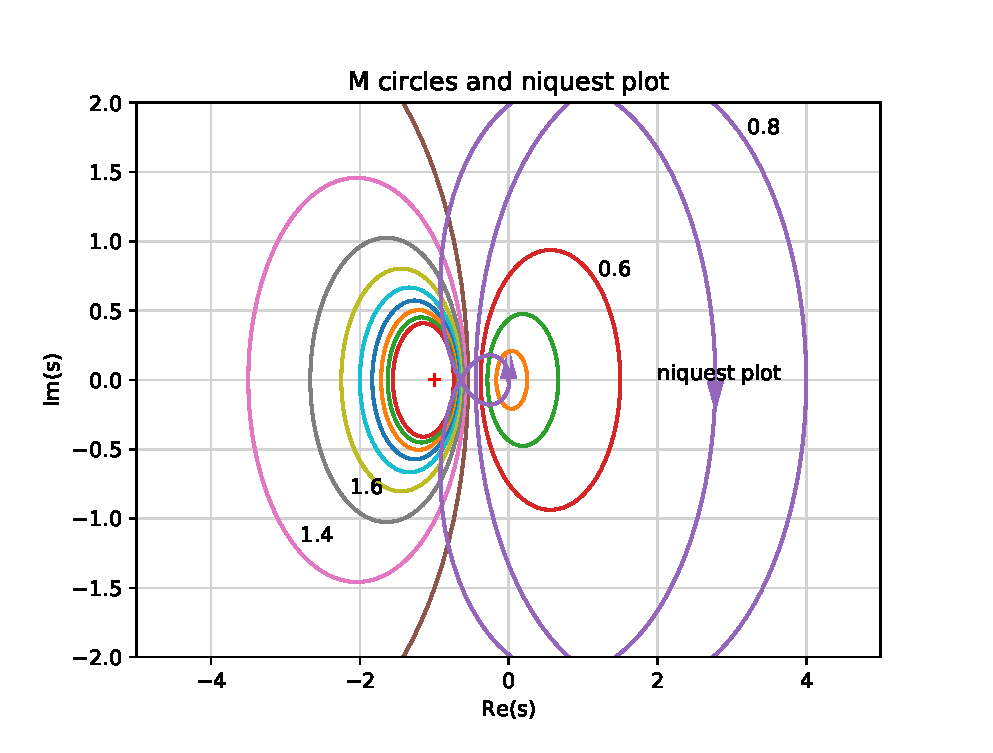
\includegraphics[width=\columnwidth]{./figs/ee18btech11027/M_circles.eps} 
\caption{}
\label{fig:ee18btech11027}
\end{figure}

For different values of M,it represents a family of circles.
The intersection of niquest plot with M circles plot gives the magnitude plot of closed loop system.\\
B. phase is given by -
\begin{align}
    \phi = \arctan\frac{y}{x} - \arctan\frac{y}{1+x}\\
    \tan\phi = \frac{y}{x^2} + x + y^2
\end{align}
substituting \tan\phi = N 

\begin{align}
    N = \frac{y}{x^2} + x + y^2
\end{align}

\begin{figure}[!ht]
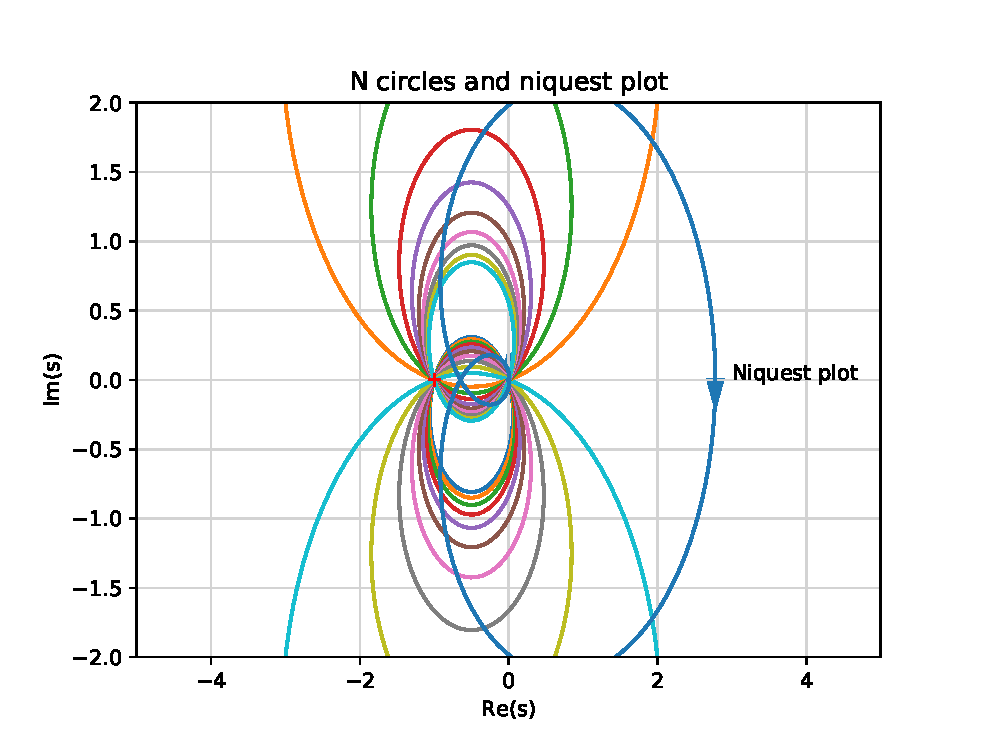
\includegraphics[width=\columnwidth]{./figs/ee18btech11027/N_circles.eps} 
\caption{}
\label{fig:ee18btech11027}
\end{figure}

For different values of N,it represents a family of circles.
The intersection of niquest plot with N circles plot gives the phase plot of closed loop system.\\

Hence closed loop frequency response is -

\begin{figure}[!ht]
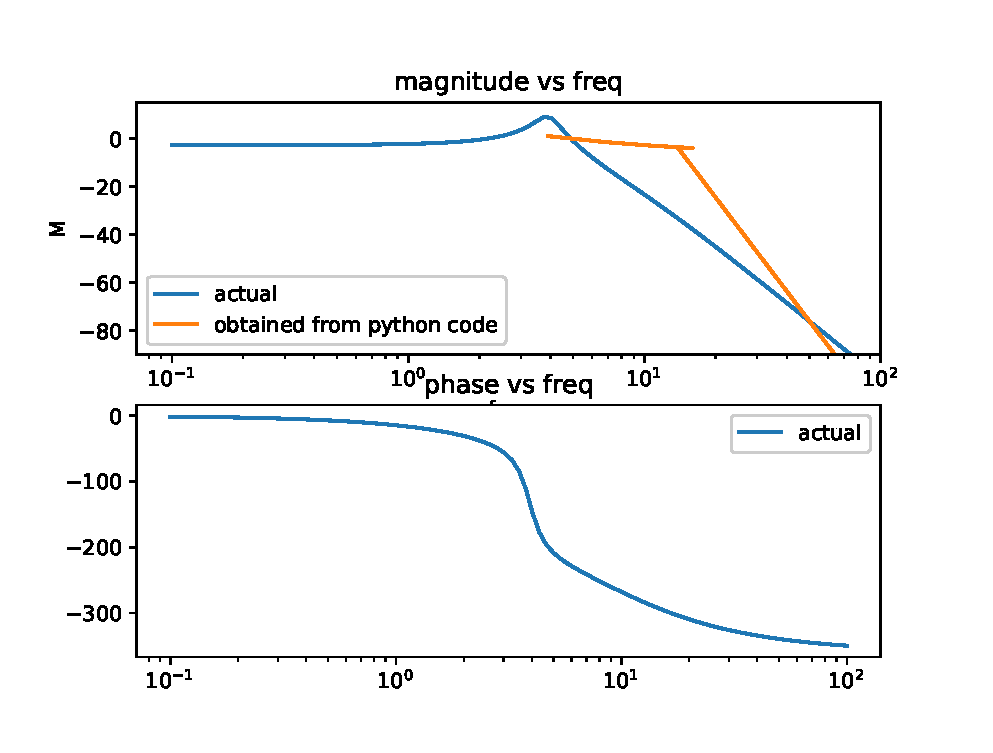
\includegraphics[width=\columnwidth]{./figs/ee18btech11027/plot.eps} 
\caption{}
\label{fig:ee18btech11027}
\end{figure}

\end{enumerate}
